%
\documentclass[12pt,notitlepage]{article}
\usepackage{amssymb}
\usepackage{amsmath}
\usepackage{yhmath}
\usepackage{graphicx}
\usepackage{epstopdf}
\usepackage{pdflscape}
\usepackage{tabularx}
\usepackage{longtable}
\usepackage{array}
\usepackage{dsfont}
\usepackage{float}
\usepackage{booktabs}
\usepackage{tikz}
\usepackage{marvosym}
\usepackage{multirow}
\usepackage{pdflscape}
\usepackage[hyphenbreaks]{breakurl}
\usepackage[hyphens]{url}
\usepackage{setspace}
\usepackage{epigraph}
\usepackage{bm}
\usepackage{textcomp}
\usepackage{diagbox}
\usepackage{bbm}
\usepackage{verbatim}
\usepackage[framemethod=tikz]{mdframed}
\usepackage{subcaption}
\usepackage{caption}
\usepackage{lipsum}
\usepackage{longtable}
\usepackage[shortlabels]{enumitem}
\setlength{\epigraphrule}{0pt}
\setlength\parindent{0pt}
\renewcommand{\baselinestretch}{1.25}
\usepackage{geometry}

\setcounter{MaxMatrixCols}{10}

\newcolumntype{L}[1]{>{\raggedright\let\newline\\\arraybackslash\hspace{0pt}}m{#1}}
\newcolumntype{C}[1]{>{\centering\let\newline\\\arraybackslash\hspace{0pt}}m{#1}}

\usepackage{natbib,hyperref}
\bibliographystyle{chicago}  

\newcommand{\I}{\mathbb{I}}
\newcommand{\E}{\mathbb{E}}
\newcommand{\Ll}{\mathrm{L}}
\renewcommand{\L}{\mathbb{L}}
\newcommand{\Var}{\mathrm{Var}}
\newcommand{\Cov}{\mathrm{Cov}}
\newcommand{\Corr}{\mathrm{Corr}}
\newcommand{\Prob}{\mathbb{P}}
\newcommand{\supp}{\mathrm{supp}}
\newcommand{\notimplies}{\mathrel{{\ooalign{\hidewidth$\not\phantom{=}$\hidewidth\cr$\implies$}}}}
\newcommand{\var}{\mathrm{var}}
\newcommand{\cov}{\mathrm{cov}}
\newcommand{\corr}{\mathrm{corr}}

\topmargin=-1.5cm \textheight=23cm \oddsidemargin=0.5cm
\evensidemargin=0.5cm \textwidth=15.5cm
\newtheorem{ass}{Assumption}
\newtheorem{definit}{Definition}
\newtheorem{prop}{Proposition}
\newtheorem{thm}{Theorem}
\newtheorem{lem}{Lemma}
\newtheorem{conj}{Conjecture}
\newtheorem{cor}{Corollary}
\newtheorem{rem}{Remark}
\renewcommand{\thesubsection}{\arabic{section}.\arabic{subsection}}
\renewcommand{\thesubsubsection}{\arabic{section}.\arabic{subsection}.\arabic{subsubsection}}

\newcommand\independent{\protect\mathpalette{\protect\independenT}{\perp}}
\def\independenT#1#2{\mathrel{\rlap{$#1#2$}\mkern2mu{#1#2}}}

\usepackage{epsfig,hyperref}

\hypersetup{
	pdftitle={ECON 21030 Template Latex Code},    % title
	pdfauthor={Francesco Ruggieri},     % author
	pdfnewwindow=true,      % links in new window
	colorlinks=true,       % false: boxed links; true: colored links
	linkcolor=blue,          % color of internal links
	citecolor=red,        % color of links to bibliography
	filecolor=black,      % color of file links
	urlcolor=blue           % color of external links
}

\allowdisplaybreaks

\title{Latex template} 
\begin{document}
	\maketitle
	
	\tableofcontents
	
	\section{Section} 
	This is a section.
	
	\subsection{Subsection}
	This is a subsection
	
	\section{Table}

	\begin{table}[H]
		\setlength{\tabcolsep}{3pt}
			\caption{Sample table} 
			\begin{tabular}{@{}  ccccccccccc}
				% latex table generated in R 4.2.3 by xtable 1.8-4 package
% Tue Dec 26 13:32:02 2023
degree\_bach & public & min & p10 & p25 & median & p75 & p90 & max & mean & CV \\ 
  \hline
  0 &   0 & 0.00 & 2.00 & 9.00 & 20.22 & 242.14 & 263.86 & 294.73 & 110.16 & 1.09 \\ 
    0 &   1 & 4.00 & 366.37 & 591.84 & 1071.10 & 1643.71 & 3509.92 & 6133.81 & 1448.86 & 0.87 \\ 
    1 &   0 & 0.00 & 224.18 & 503.06 & 786.81 & 1355.94 & 1620.66 & 1890.17 & 898.44 & 0.56 \\ 
    1 &   1 & 1708.84 & 4352.22 & 6468.64 & 8907.82 & 14235.11 & 17537.12 & 18351.72 & 10220.19 & 0.49 \\ 
   \hline

			\end{tabular}
	\end{table}
	
	
	\section{Regression table}
	
% Table created by stargazer v.5.2.3 by Marek Hlavac, Social Policy Institute. E-mail: marek.hlavac at gmail.com
% Date and time: Tue, Dec 26, 2023 - 13:35:30
\begin{table}[H] \centering 
  \caption{enrollment number by perivous year avg grant amount} 
  \label{} 
\begin{tabular}{@{\extracolsep{5pt}}lcccc} 
\\[-1.8ex]\hline 
\hline \\[-1.8ex] 
 & \multicolumn{4}{c}{\textit{Dependent variable:}} \\ 
\cline{2-5} 
\\[-1.8ex] & \multicolumn{4}{c}{enroll\_ftug} \\ 
\\[-1.8ex] & (1) & (2) & (3) & (4)\\ 
\hline \\[-1.8ex] 
 lag\_avg\_grant & 0.094$^{***}$ & 0.063$^{***}$ & 0.027$^{**}$ & 0.027$^{**}$ \\ 
  & (0.019) & (0.017) & (0.013) & (0.013) \\ 
  & & & & \\ 
 public &  & 629.694$^{***}$ & 396.437$^{***}$ & 396.332$^{***}$ \\ 
  &  & (49.807) & (57.734) & (57.870) \\ 
  & & & & \\ 
 degree\_bach &  &  & 66.062 & 66.103 \\ 
  &  &  & (56.349) & (56.481) \\ 
  & & & & \\ 
 as.factor(Year)2011 &  &  &  & $-$24.496 \\ 
  &  &  &  & (65.261) \\ 
  & & & & \\ 
 as.factor(Year)2012 &  &  &  & $-$60.909 \\ 
  &  &  &  & (65.278) \\ 
  & & & & \\ 
 as.factor(Year)2013 &  &  &  & $-$62.513 \\ 
  &  &  &  & (65.267) \\ 
  & & & & \\ 
 as.factor(Year)2014 &  &  &  & $-$58.042 \\ 
  &  &  &  & (65.298) \\ 
  & & & & \\ 
 as.factor(Year)2015 &  &  &  & $-$1.916 \\ 
  &  &  &  & (65.334) \\ 
  & & & & \\ 
 public:degree\_bach &  &  & 1,479.567$^{***}$ & 1,479.431$^{***}$ \\ 
  &  &  & (91.211) & (91.420) \\ 
  & & & & \\ 
 Constant & 148.969$^{*}$ & 4.227 & 106.951 & 141.089$^{*}$ \\ 
  & (85.005) & (77.001) & (67.632) & (79.160) \\ 
  & & & & \\ 
\hline \\[-1.8ex] 
Observations & 647 & 647 & 647 & 647 \\ 
R$^{2}$ & 0.037 & 0.228 & 0.547 & 0.548 \\ 
Adjusted R$^{2}$ & 0.035 & 0.226 & 0.544 & 0.542 \\ 
\hline 
\hline \\[-1.8ex] 
\textit{Note:}  & \multicolumn{4}{r}{$^{*}$p$<$0.1; $^{**}$p$<$0.05; $^{***}$p$<$0.01} \\ 
\end{tabular} 
\end{table} 

	

	\section{Graphs}
	This is a sample plot.
	
	\begin{figure}[H]
		\centering
		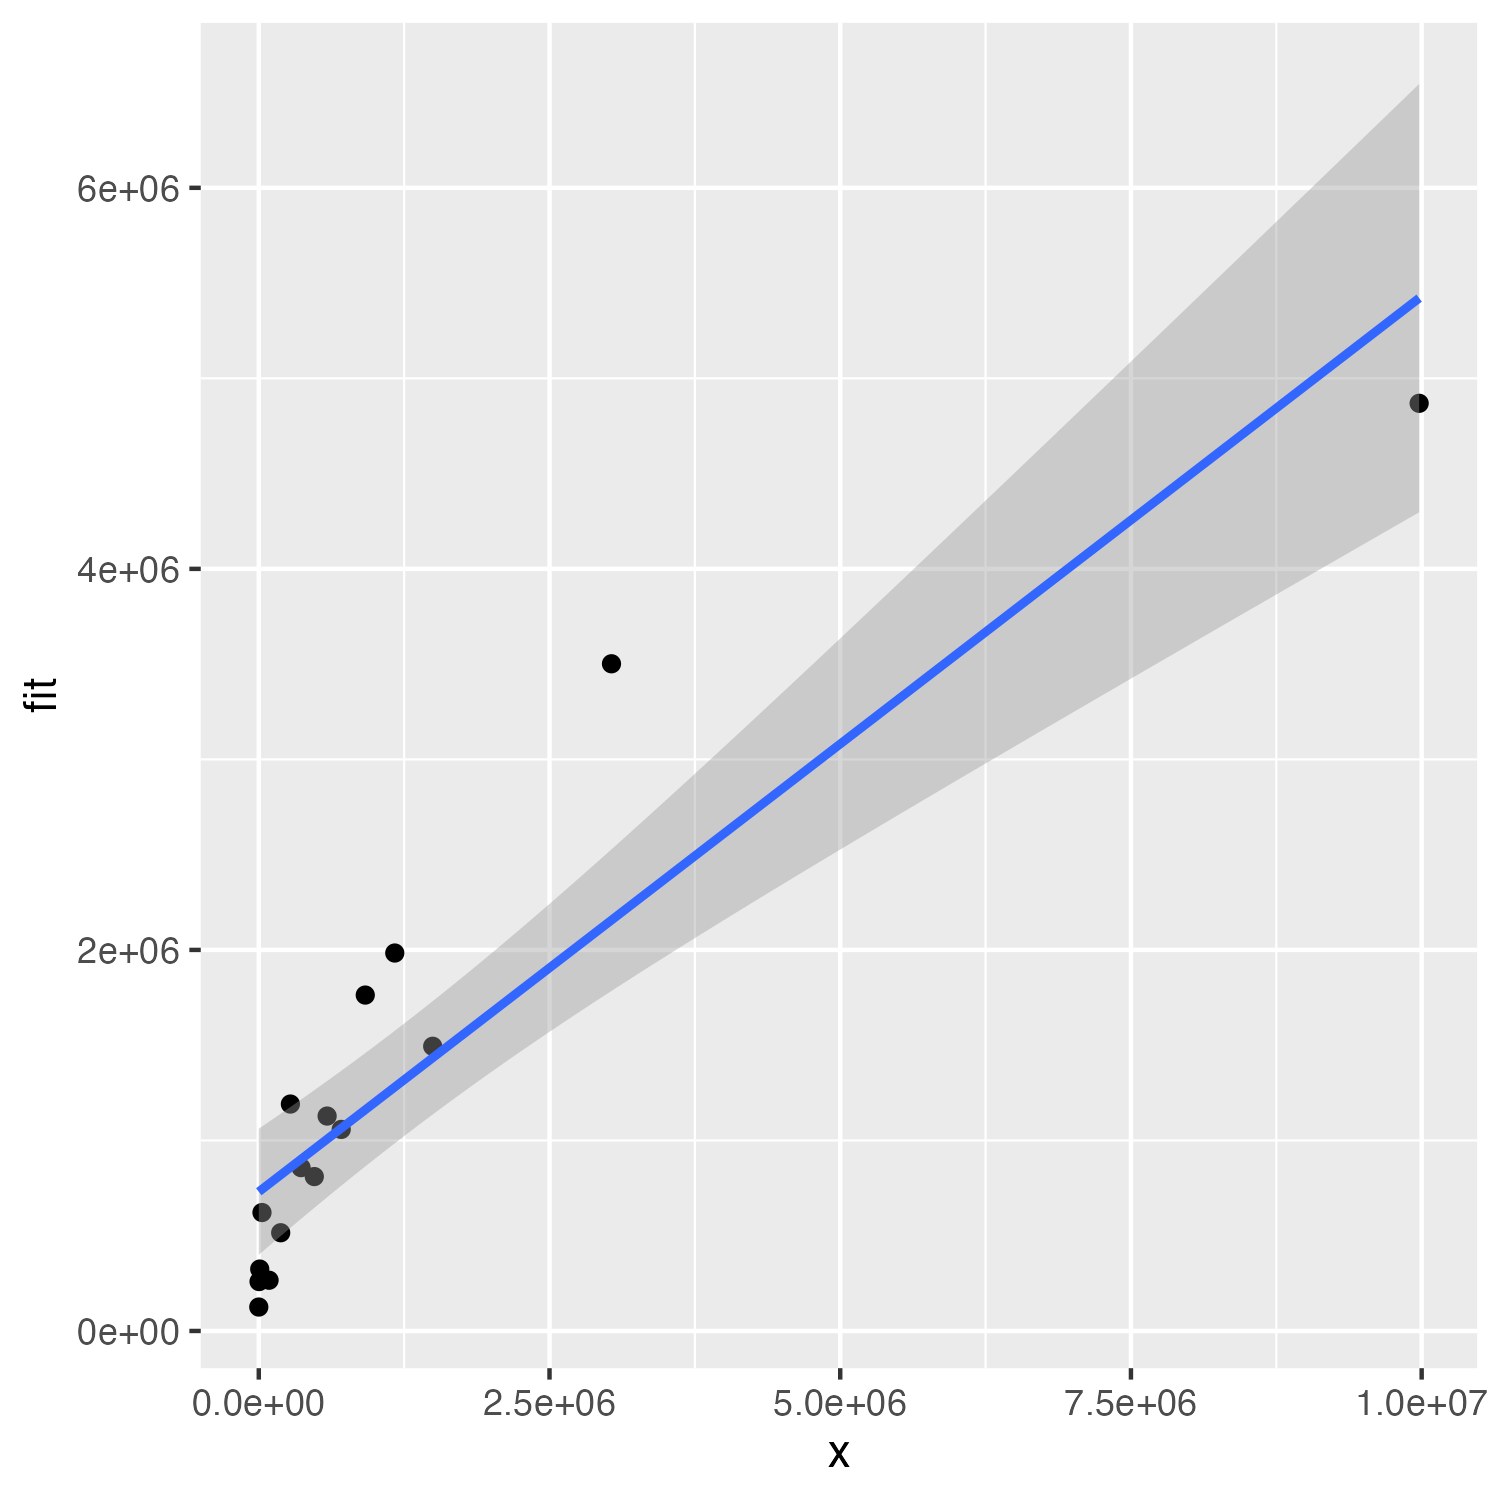
\includegraphics[width=\textwidth]{../figure/plot.png}
		\caption{Plot}
	\end{figure}


	
	
\end{document}
